\documentclass[11pt,a4paper]{article}
\usepackage[utf8]{inputenc}
\usepackage[T1]{fontenc}
\usepackage{lmodern}
\usepackage[french]{babel}
\usepackage{amsmath,amssymb}
\usepackage{graphicx}
\usepackage{booktabs}
\usepackage[margin=2.3cm]{geometry}
\usepackage{xcolor}
\usepackage[hidelinks]{hyperref}
\usepackage{tcolorbox}
\tcbuselibrary{skins}
\newtcolorbox{resultat}{colback=blue!4,colframe=blue!50!black,boxrule=0.6pt,arc=2pt,left=6pt,right=6pt,top=4pt,bottom=4pt}
\newtcolorbox{intuition}{colback=orange!5,colframe=orange!60!black,boxrule=0.6pt,arc=2pt,left=6pt,right=6pt,top=4pt,bottom=4pt}
\graphicspath{{../results/}}
\newcommand{\DE}{\Delta E}

\title{\textbf{Physique statistique des échecs}\\[2pt]\large Où en est le projet ? — récapitulatif pédagogique}
\author{Projet \texttt{chess-physics}}
\date{20 novembre 2026}

\begin{document}
\maketitle

\begin{abstract}
On traite le choix d'un coup aux échecs comme un problème de physique statistique : chaque coup possible est un
« état », sa perte par rapport au meilleur coup (mesurée par le moteur Stockfish) est son « énergie », et le joueur
choisit avec une certaine « température ». Sur environ 18\,000 positions de parties en ligne (Lichess), nous
mesurons la loi de choix, ce qui fait varier la température, et testons des relations classiques de la physique
statistique (fluctuation-dissipation, chaleur spécifique). Ce document résume les résultats, sans prérequis
autres que des notions de probabilités.
\end{abstract}

\tableofcontents
\newpage

%=====================================================================
\section{L'idée en une page}

Dans une position d'échecs, le joueur au trait a en moyenne une trentaine de coups légaux. Un moteur d'échecs
(Stockfish) attribue à chacun une évaluation $e_i$ en \emph{centipions} (cp ; 100 cp $\approx$ un pion d'avance).
On appelle \textbf{énergie} d'un coup sa perte par rapport au meilleur :
\begin{equation}
  \DE_i = \max_j e_j - e_i \;\ge 0 .
\end{equation}
Le meilleur coup a l'énergie $0$ ; une gaffe qui perd une pièce a une énergie de plusieurs centaines de cp.

\begin{intuition}
\textbf{Analogie physique.} Une molécule en contact avec un thermostat n'occupe pas toujours son état d'énergie
minimale : elle visite aussi des états plus énergétiques, d'autant plus souvent que la température $T$ est élevée
(loi de Boltzmann, $p_i \propto e^{-E_i/T}$). Un joueur humain ne joue pas toujours le meilleur coup ; il
« visite » des coups moins bons, d'autant plus qu'il est faible ou pressé. La \emph{température} mesure ce
« bruit » de décision : $T = 0$ serait un joueur parfait, $T$ grand un joueur qui joue au hasard.
\end{intuition}

Les questions du projet :
\begin{enumerate}
  \item \textbf{Forme de la loi} : les choix suivent-ils vraiment une loi de Boltzmann ?
  \item \textbf{Mécanisme} : le joueur considère-t-il tous les coups, ou seulement quelques-uns ?
  \item \textbf{Ce qui fait varier la température} : niveau (Elo), pendule, phase de jeu, score, type de position,
        joueur individuel.
  \item \textbf{Cohérence thermodynamique} : une seule température suffit-elle (fluctuation-dissipation,
        chaleur spécifique) ?
  \item \textbf{Énergie contre entropie} : les joueurs cherchent-ils à garder des options (stratégie) ou à
        en priver l'adversaire (tactique) ?
\end{enumerate}

%=====================================================================
\section{Données et méthode}

\paragraph{Parties.} Base publique Lichess d'octobre 2026 (les 2 premiers Go du fichier mensuel), parties
\emph{Blitz} (3 à 5 min) et \emph{Rapid} (10 à 15 min), classées en tranches d'Elo de 200 points de 800 à 2600,
les deux joueurs étant dans la même tranche. Environ 1000 positions par case (cadence $\times$ tranche),
\textbf{une seule position par partie} (tirée au hasard après le 10\textsuperscript{e} demi-coup), ce qui rend les
observations indépendantes.

\paragraph{Évaluations.} Stockfish 18 évalue \emph{tous} les coups légaux de chaque position (profondeur 12),
soit le « spectre » complet des énergies. Les positions déjà jouées d'avance de plus de 500 cp sont exclues.

\paragraph{Ajustement.} Pour un modèle de choix $p_i(\theta)$, on maximise la vraisemblance
\begin{equation}
  \mathcal{L}(\theta) = \sum_{n=1}^{N} \log p_{i_n}(\theta),
\end{equation}
où $i_n$ est le coup réellement joué dans la position $n$. Les intervalles de confiance (IC à 95 \%) viennent
du \emph{bootstrap} (on rééchantillonne les parties) ; deux modèles emboîtés se comparent par le
\emph{rapport de vraisemblance} $\mathrm{LR} = 2(\mathcal{L}_1 - \mathcal{L}_0)$, qui suit une loi du $\chi^2$
sous l'hypothèse du modèle simple.

%=====================================================================
\section{Résultat 1 : la loi de choix n'est pas de Boltzmann}

Le modèle le plus simple est la loi de Boltzmann (en économie : le \emph{logit}) :
\begin{equation}
  p_i = \frac{e^{-\DE_i/T}}{\sum_j e^{-\DE_j/T}} .
\end{equation}
Elle donne une température qui décroît avec le niveau, de $T\approx 110$ cp (Elo 800-1800) à
$T \approx 45$ cp (Elo 2400-2600). Mais elle est \textbf{rejetée partout} au profit d'une
\textbf{exponentielle étirée} :
\begin{equation}
  p_i \propto \exp\!\left[-\left(\frac{\DE_i}{s}\right)^{c}\right],
  \qquad c \approx 0{,}5 .
\end{equation}
$s$ (en cp) joue le rôle de la température, $c$ décrit la \emph{forme}. Pour $c=1$ on retrouve Boltzmann.
On trouve $c \approx 0{,}5$ dans toutes les cases (LR de 108 à 290 contre Boltzmann), résultat robuste au bruit
d'évaluation (profondeur 20) et au spectre complet. Ce modèle est celui de Regan et Haworth (2011) :
nos données le confirment indépendamment.

\begin{intuition}
$c < 1$ signifie que la probabilité baisse \emph{vite} pour les petites pertes (forte prime au meilleur coup) puis
\emph{lentement} pour les grosses : les gaffes énormes sont bien plus fréquentes que ne le voudrait Boltzmann.
\end{intuition}

\begin{figure}[h]
  \centering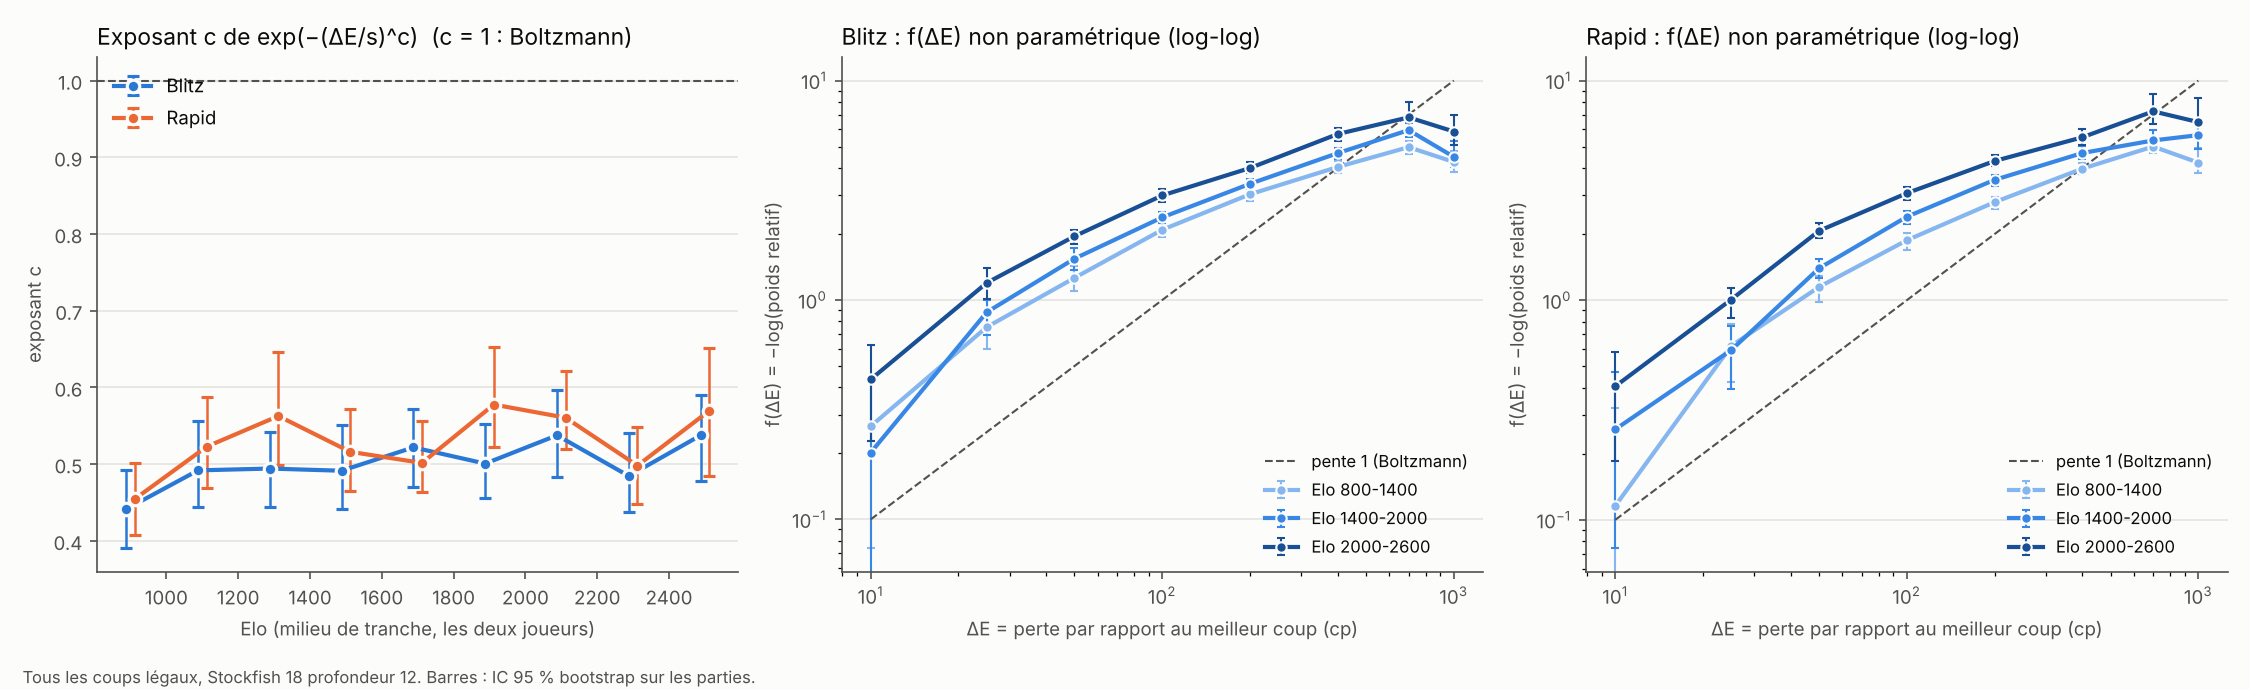
\includegraphics[width=\linewidth]{spectrum.png}
  \caption{Exposant $c$ par case et forme non paramétrique $f(\DE)=-\log p$ : $f$ croît comme $\DE^{0{,}6}$.}
\end{figure}

%=====================================================================
\section{Résultat 2 : on ne regarde qu'une partie des coups}

La loi précédente, ajustée sur les 5 meilleurs coups, \emph{surprédit} la fréquence des coups joués hors de ce
top~5 (prédit 25-57 \%, observé 17-37 \%). Les mauvais coups ne sont pas « accessibles » comme dans un gaz :
le joueur n'en envisage qu'un sous-ensemble. D'où un \textbf{modèle à deux étages} :
\begin{enumerate}
  \item le joueur envisage les $K$ coups les plus « saillants » ($K$ aléatoire, de loi $\pi_K$ ajustée ; le rang
        Stockfish sert d'approximation de la saillance) ;
  \item il choisit parmi eux selon l'exponentielle étirée.
\end{enumerate}
\begin{equation}
  p_i = w_i \sum_{K} \pi_K \,\frac{\mathbf{1}[\mathrm{rang}(i) < K]}{\sum_{j:\,\mathrm{rang}(j)<K} w_j},
  \qquad w_i = e^{-(\DE_i/s)^c}.
\end{equation}

\begin{resultat}
Le modèle à deux étages est bien meilleur (LR de 38 à 167) et reproduit le taux de coups hors top~5.
Le nombre effectif de coups envisagés, $\Omega_\text{eff} = \mathbb{E}[\min(K,N)]$, passe d'environ
\textbf{20} (Elo 900) à \textbf{14} (Elo 2300-2500) sur $\sim$33 coups légaux : les forts joueurs « élaguent »
davantage, comme l'avait observé de Groot chez les maîtres.
\end{resultat}

\begin{figure}[h]
  \centering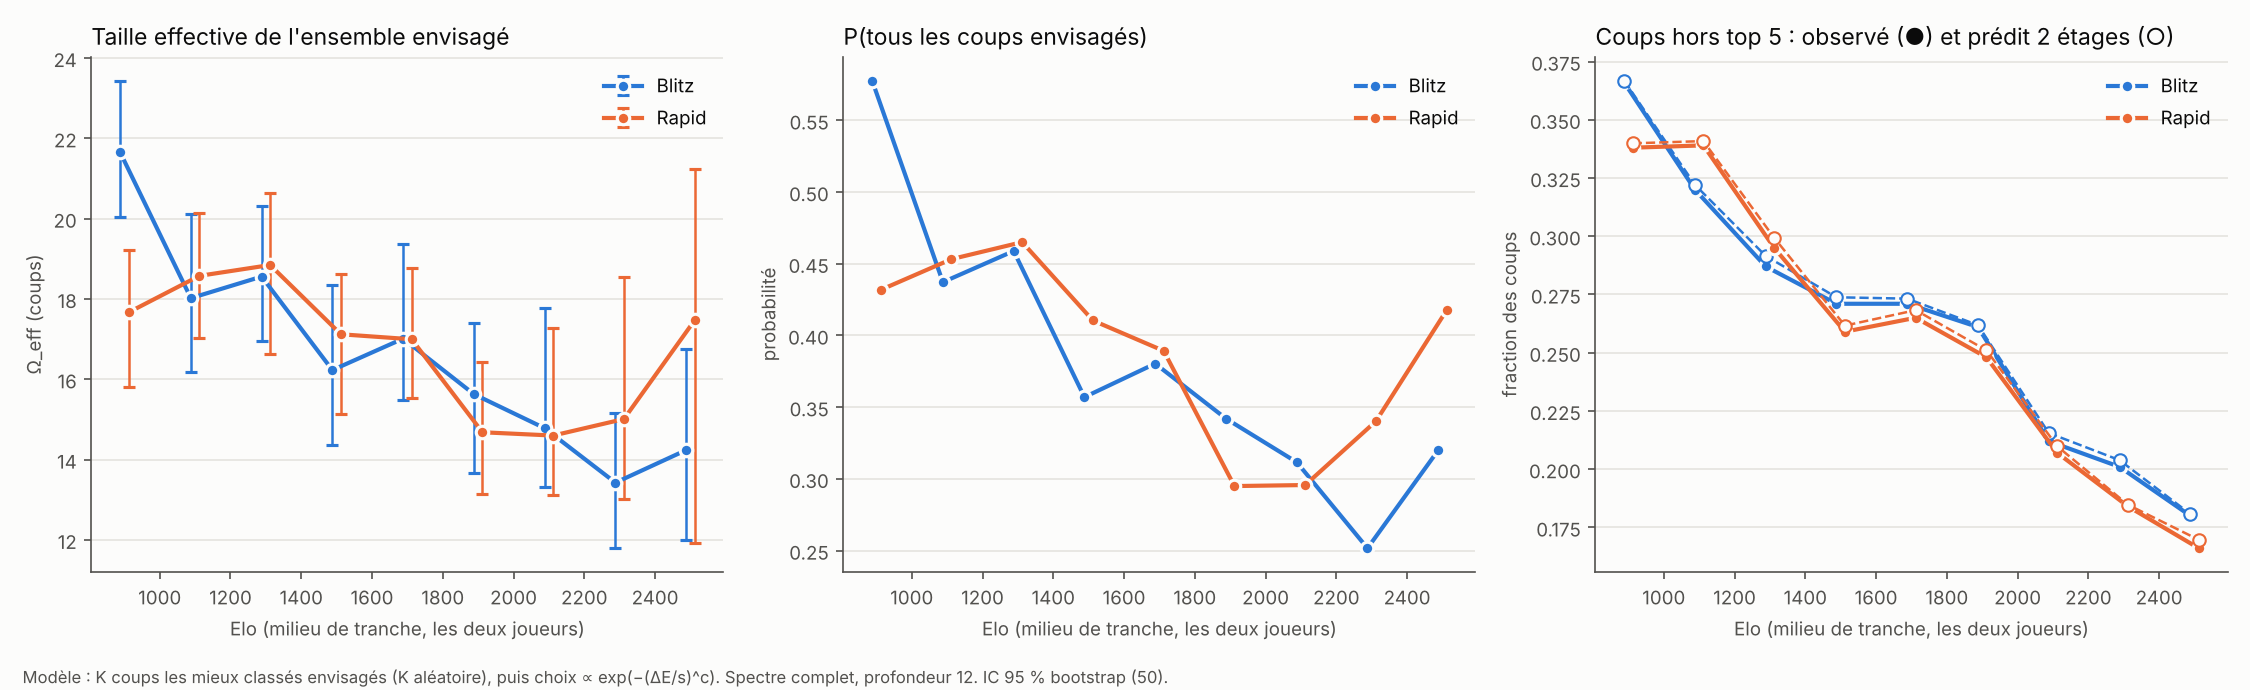
\includegraphics[width=0.95\linewidth]{attention.png}
  \caption{Modèle à deux étages : nombre effectif de coups envisagés $\Omega_\text{eff}$ selon l'Elo.}
\end{figure}

%=====================================================================
\section{Résultat 3 : qu'est-ce qui fait varier la température ?}

On fixe $c$ et on écrit l'échelle $s$ comme un produit de facteurs (modèle additif en logarithme) :
\begin{equation}
  \log s = a(\text{Elo}) + d(\text{demi-coup}) + e(\text{score}) + g(\text{écart}) + h\cdot\mathbf{1}[\text{échec}] + \dots
\end{equation}
Chaque facteur se teste en le retirant (rapport de vraisemblance). Les effets sont exprimés en
\emph{rapports} de $s$ : « $\times 2$ » veut dire deux fois plus « chaud ».

\begin{center}
\begin{tabular}{lll}
\toprule
Facteur & Effet sur $s$ (température) & Solidité \\
\midrule
Niveau (Elo 800 $\to$ 2500) & $\times 1/2{,}8$ (plus froid) & très forte \\
Avancement (demi-coup $<30 \to >70$) & $\times 2$ Blitz, $\times 1{,}5$ Rapid & $p<10^{-13}$ \\
Pendule, à phase fixée & aucun effet propre (p = 0,22 et 0,57) & -- \\
Roi en échec & $\times 4{,}5$ Blitz, $\times 2{,}7$ Rapid & $p<10^{-8}$ \\
Score (proba.~de gain) : mené $>300$ cp & $\times 0{,}6$ (plus froid) & $p<10^{-17}$ \\
Score : mène $>300$ cp & $\times 1{,}2$ (plus chaud) & idem \\
Un coup se détache (écart $>30$ cp) & $\times 1{,}2$ & $p\sim 10^{-3}$ \\
Joueur individuel (même Elo) & dispersion $<12\,\%$ & voir §7 \\
\bottomrule
\end{tabular}
\end{center}

\paragraph{Pendule ou phase de jeu ?} Quand il reste peu de temps, la partie est avancée (corrélation $-0{,}84$
entre temps restant et numéro de coup). L'effet apparent de la pendule ($\times 2{,}2$ en Blitz) disparaît
quand on contrôle le numéro de coup : c'est l'\textbf{avancement de la partie} qui « chauffe » le joueur
(fatigue, complexité ou temps déjà consommé : à démêler), pas l'horloge en soi.

\begin{figure}[h]
  \centering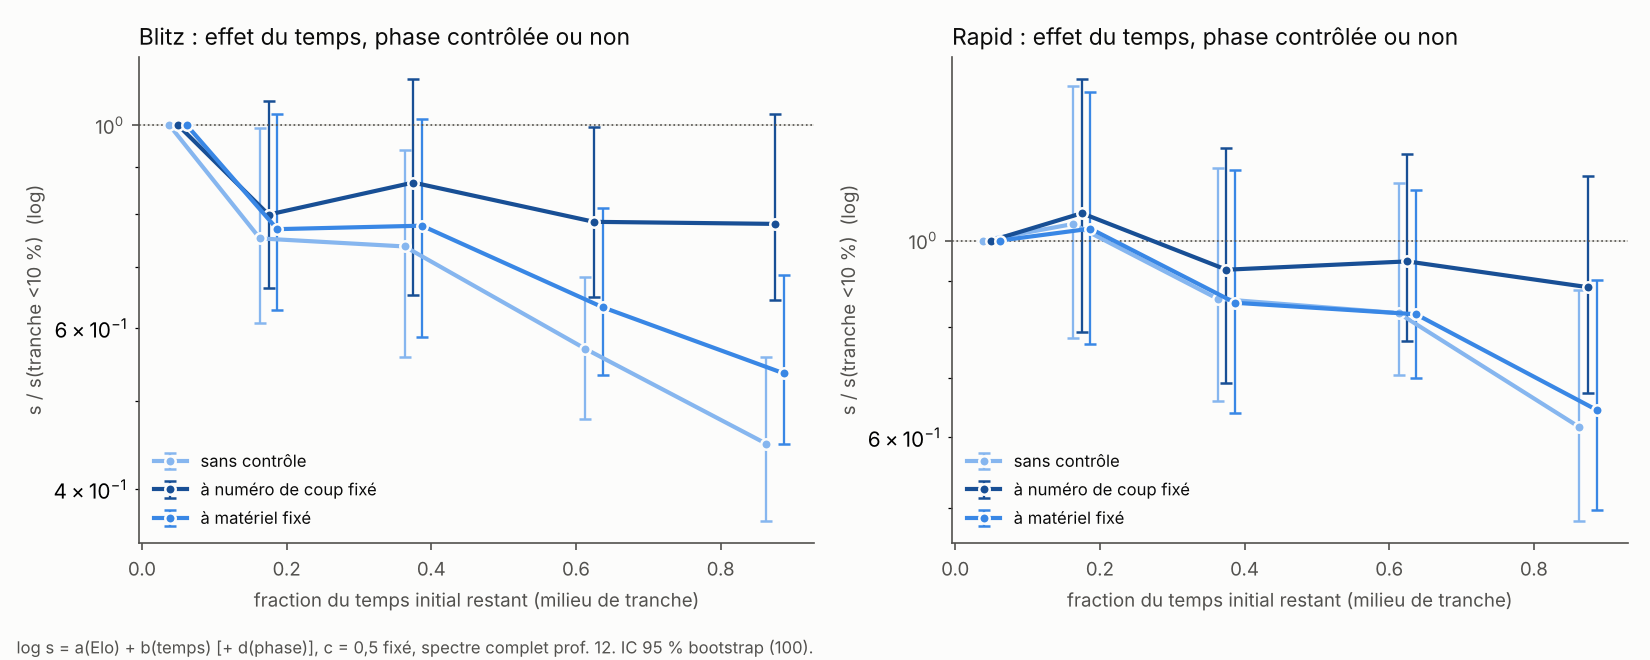
\includegraphics[width=0.9\linewidth]{phase.png}
  \caption{Effet du temps restant sur $s$ sans contrôle, puis à numéro de coup fixé (l'effet disparaît)
  et à matériel fixé.}
\end{figure}

\paragraph{Le score.} En probabilité de gain (l'énergie qui décrit le mieux les choix), le joueur
\emph{mené} joue plus froid (il se bat) et celui qui \emph{mène} accepte de petites pertes (il simplifie).

%=====================================================================
\section{Résultat 4 : une seule température suffit-elle ?}

\subsection{Fluctuation-dissipation}
En physique, pour un système à l'équilibre à température $T$, la réponse de l'énergie moyenne à la température
est fixée par ses fluctuations :
\begin{equation}
  \frac{\partial \langle E\rangle}{\partial T} = \frac{\operatorname{Var}(E)}{T^2}
  \qquad\Longleftrightarrow\qquad
  \frac{\partial \langle H\rangle}{\partial \beta} = -\operatorname{Var}(H) .
\end{equation}
Pour un logit $p_i \propto e^{-\beta H_i}$, l'ajustement fixe $\beta$ par l'énergie \emph{moyenne} ; la relation
prédit alors les \emph{fluctuations}. On mesure le rapport
\begin{equation}
  R = \frac{\sum_n \left(H_{\text{obs},n} - \langle H\rangle_n\right)^2}{\sum_n \operatorname{Var}_n(H)} ,
\end{equation}
qui vaut 1 si une seule température rend compte des choix.

\begin{resultat}
Boltzmann ($H = \DE$) : $R = 2{,}9$, violation massive. Exponentielle étirée : $R = 1{,}5$ ; dans la variable
$H = \DE^{0{,}5}$, les deux températures (moyenne et fluctuations) coïncident à 2 \% près. Modèle à deux
étages : $R = 1{,}26\;[1{,}18 ; 1{,}34]$ : il reste $\sim$25 \% de fluctuations en excès.
\end{resultat}

\subsection{Chaleur spécifique}
La chaleur spécifique (sans dimension) mesure la sensibilité du choix à la température :
\begin{equation}
  C = \beta^2 \operatorname{Var}(H) = -\beta\,\frac{\partial\langle H\rangle}{\partial \beta},
  \qquad H = \DE^c,\; \beta = s^{-c}.
\end{equation}
\begin{resultat}
\begin{itemize}
  \item Sur l'ensemble des positions, $C(s)$ culmine à $s^* \approx 10$-$13$ cp, juste sous la plage des
        joueurs humains (12-31 cp) : tous les niveaux sont sur le plateau du maximum.
  \item Le pic dépend du type de position : $s^*\approx 3$-$5$ cp quand plusieurs coups se valent, mais
        $s^* \approx 20$ cp quand un coup se détache de 100 à 300 cp. \textbf{Ce sont ces positions « à coup
        qui se détache » qui discriminent les niveaux} ; les positions calmes sont « saturées ».
  \item L'excès de fluctuations ($R>1$) est concentré dans les positions à \emph{coup unique} (écart $>300$ cp,
        $C_\text{obs}/C_\text{modèle}\approx 2$) : on y trouve le coup ou on gaffe lourdement, un comportement
        en tout-ou-rien que la loi continue ne capte pas.
\end{itemize}
\end{resultat}

\begin{figure}[h]
  \centering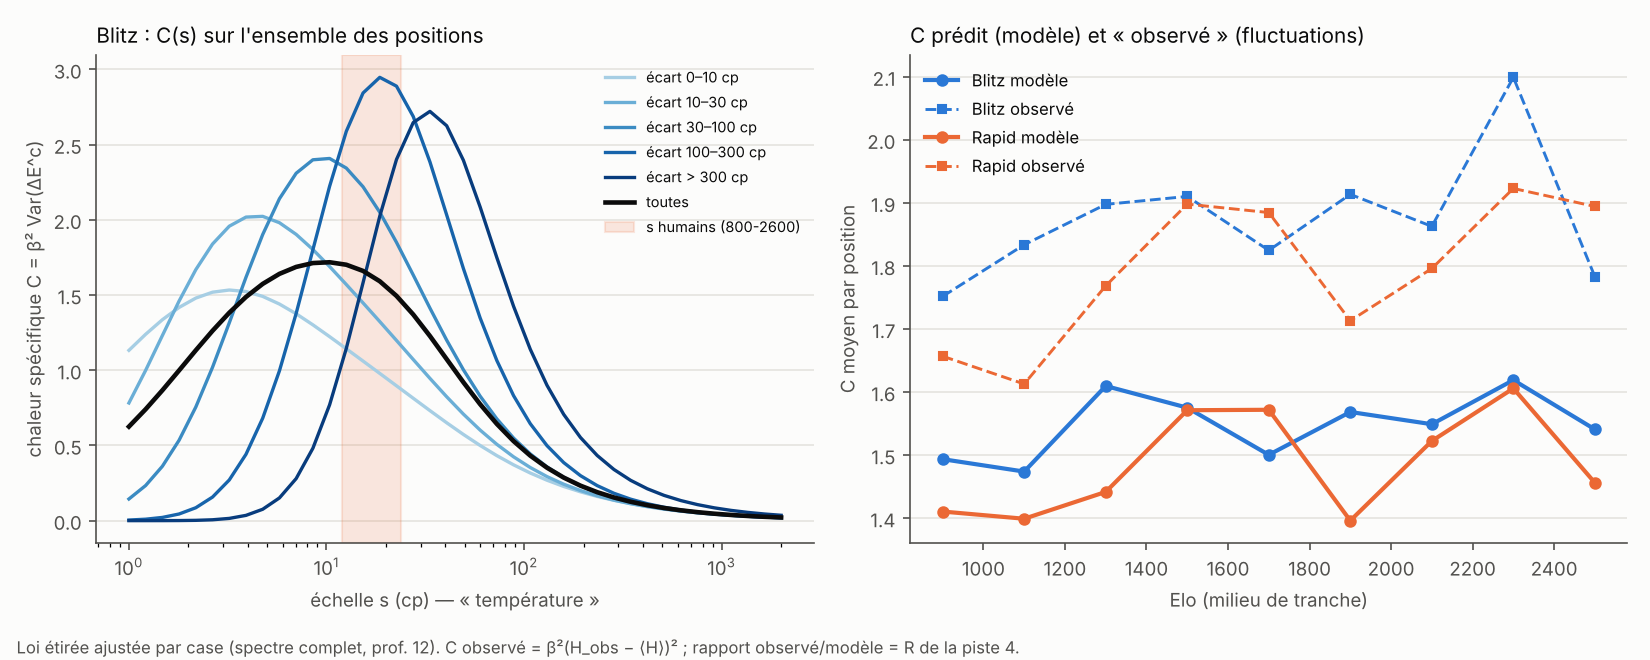
\includegraphics[width=\linewidth]{heat.png}
  \caption{Gauche : chaleur spécifique $C(s)$ par type de position, bande orange = températures humaines.
  Droite : $C$ prédit et observé selon l'Elo.}
\end{figure}

%=====================================================================
\section{Résultat 5 : pas de « désordre » entre joueurs}

Deux joueurs de même Elo ont-ils la même température ? Nouvel échantillon : 160 joueurs Blitz actifs, 25
positions chacun. Modèle à effets aléatoires :
\begin{equation}
  \log s_n = a(\text{Elo}) + d(\text{demi-coup}) + h\cdot\mathbf{1}[\text{échec}] + u_{\text{joueur}(n)},
  \qquad u \sim \mathcal{N}(0,\sigma^2).
\end{equation}
\begin{resultat}
$\sigma = 0$, IC 95 \% $[0 ; 0{,}12]$ (méthode validée sur simulation : $\sigma = 0{,}3$ est bien retrouvé). À Elo,
phase et échec fixés, les joueurs ont la même température à $\pm 12$ \% près, alors que $s$ varie d'un facteur
2,8 entre 800 et 2200 Elo : \textbf{l'Elo est presque une description complète de la « température »}.
L'excès de fluctuations du §6 vient donc des positions, pas des joueurs.
\end{resultat}

%=====================================================================
\section{En cours : énergie contre entropie (tactique contre stratégie)}
\subsection{La question}
Le joueur au trait cherche-t-il seulement à minimiser l'énergie (jouer le meilleur coup), ou tient-il aussi compte
du \emph{nombre d'options} que laisse chaque coup ? Pour un coup $i$, on évalue (Stockfish, profondeur 10) :
\begin{itemize}
  \item la position \emph{fille} (adversaire au trait) : $S_\text{adv}(i) = \log N_\text{bons}$, où $N_\text{bons}$
        est le nombre de coups de l'adversaire à moins de 50 cp de son meilleur ;
  \item la position \emph{petite-fille}, après la meilleure réponse adverse : $S_\text{moi}(i)$, même définition
        pour le joueur.
\end{itemize}
$S$ est une entropie de Boltzmann, $S = \log(\text{nombre d'états accessibles})$. Garder $S_\text{moi}$ élevé,
c'est garder des options (jeu \og stratégique\fg{}) ; rendre $S_\text{adv}$ faible, c'est forcer l'adversaire à
trouver le seul bon coup (jeu \og tactique\fg{}).

\subsection{Deux modèles}
\paragraph{(A) Compromis énergie / entropie.} On ajoute l'entropie à l'« utilité » de chaque coup :
\begin{equation}
  p_i \propto \exp\!\Big[-\big(\DE_i/s\big)^{c} + \lambda_\text{moi}\, S_\text{moi}(i) + \lambda_\text{adv}\, S_\text{adv}(i)\Big].
\end{equation}
C'est l'analogue d'une \textbf{énergie libre} $F_i = E_i - \tau S_i$ : $\lambda$ fixe le taux de change entre
qualité du coup et nombre d'options.

\paragraph{(B) Énergie libre « rationnelle ».} Un joueur faillible, de température $s$, devrait évaluer une position
non par sa valeur exacte mais par sa valeur \emph{pratique} : on y retranche les erreurs qu'il risque de commettre
et on y ajoute celles que l'adversaire risque de commettre. Avec $L(\cdot) = \langle \DE\rangle$ la perte moyenne
attendue du joueur au trait (sous la loi de choix de son niveau) :
\begin{equation}
  E_i^{\text{prat}} = \DE_i + \kappa_\text{moi}\, L_\text{moi}(i) - \kappa_\text{adv}\, L_\text{adv}(i),
\end{equation}
puis la loi étirée sur $E^{\text{prat}}$. Un joueur parfaitement conscient de sa faillibilité et de celle de
l'adversaire aurait $\kappa_\text{moi} = \kappa_\text{adv} = 1$.

\subsection{Résultats du pilote (Blitz, 837 positions, 8 coups candidats)}
\begin{resultat}
\begin{itemize}
  \item \textbf{Modèle A, nettement meilleur que l'énergie seule} (LR = 55, 2 ddl, $p\sim10^{-12}$) :
        $\lambda_\text{moi} = +0{,}27 \pm 0{,}06$ (on préfère garder ses options),
        $\lambda_\text{adv} = -0{,}37 \pm 0{,}06$ (on préfère réduire celles de l'adversaire).
        Ordre de grandeur : doubler ses bonnes options « vaut » $\sim$10-15 cp, diviser par deux celles de
        l'adversaire $\sim$15 cp.
  \item Robuste : effets inchangés à capture et échec contrôlés, avec une énergie non paramétrique, et pour
        $c = 0{,}35$ à $0{,}7$. La corrélation entre $\DE$ et $S_\text{adv}$ (une gaffe laisse peu de bons coups
        à l'adversaire) joue \emph{contre} l'effet trouvé.
  \item \textbf{Niveau} : $\lambda_\text{moi}$ diminue avec l'Elo ($0{,}40 \to 0{,}15$) : les joueurs faibles tiennent
        plus à leurs options, ce qui est le sens prédit puisqu'ils sont plus « chauds » (tendance à confirmer :
        environ $2\sigma$). $\lambda_\text{adv}$ reste $\approx -0{,}3$ à $-0{,}5$.
  \item \textbf{Modèle B} : $\kappa_\text{moi} = \kappa_\text{adv} \approx 0{,}2$ (IC $[0 ; 0{,}3]$), gain faible
        (LR = 8,5) ; le joueur « rationnel » $\kappa = 1$ est rejeté (LR = 91). Les joueurs réagissent au
        \emph{nombre} de bonnes options, pas à un calcul pondéré de leurs chances d'erreur : une heuristique,
        pas une optimisation de l'énergie libre.
\end{itemize}
\end{resultat}

\begin{figure}[h]
  \centering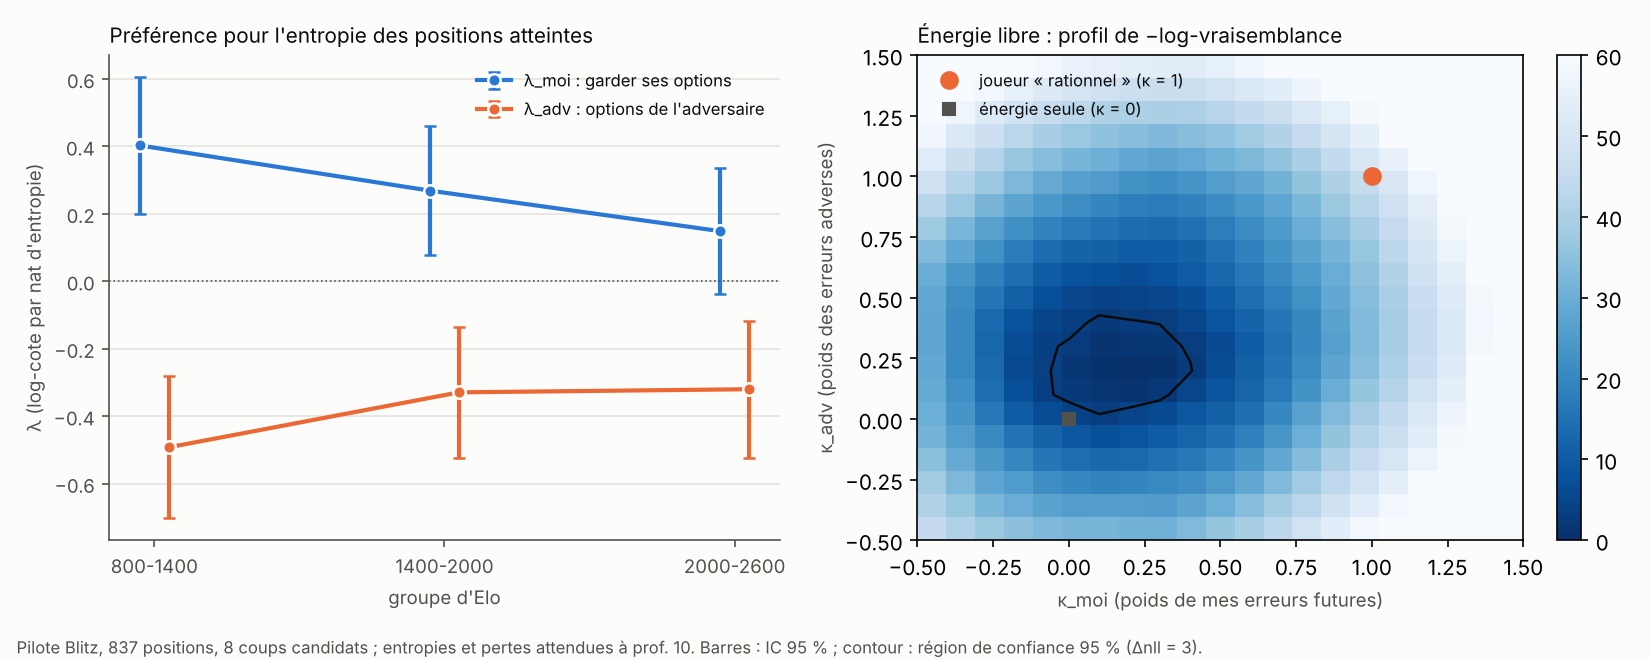
\includegraphics[width=\linewidth]{entropy.png}
  \caption{Gauche : préférences entropiques par niveau ($\lambda_\text{moi}>0$ : garder ses options ;
  $\lambda_\text{adv}<0$ : priver l'adversaire des siennes). Droite : profil de vraisemblance du modèle B ;
  le minimum est loin du point $\kappa=1$.}
\end{figure}

\paragraph{Liens avec les pistes précédentes.}
Le joueur qui mène \og simplifie\fg{} (piste 3) : c'est une réduction d'entropie, à tester directement avec
$\lambda$ selon le score. La chaleur spécifique (§6) montre que les positions où un coup se détache discriminent les
niveaux ; $S_\text{adv}$ faible fabrique précisément ce type de position pour l'adversaire. Enfin, la préférence pour
les options pourrait faire partie de la \emph{saillance} de l'étage 1 du modèle à deux étages (§4).

\paragraph{Limites du pilote.} 837 positions, Blitz seulement ; entropies mesurées à profondeur 10 ; meilleure
réponse adverse supposée pour $S_\text{moi}$ ; seuil de 50 cp arbitraire (à faire varier). Extension complète :
$\sim$9000 positions, $\approx$ 3 h de calcul.


%=====================================================================
\section{Bilan}

\subsection*{Ce qui est solide}
Loi étirée $c\approx 0{,}5$ ; mécanisme à deux étages avec $\Omega_\text{eff}$ décroissant avec l'Elo ;
effets de l'Elo, de l'avancement de la partie et de l'échec ; violation de fluctuation-dissipation pour
Boltzmann.

\subsection*{Ce qui semble original (à vérifier dans la littérature)}
\begin{itemize}
  \item absence de dispersion des températures entre joueurs de même Elo ;
  \item l'effet « pression du temps » est un effet de phase de jeu ;
  \item $\Omega_\text{eff}$ mesuré par niveau ; effet de l'échec ;
  \item fluctuation-dissipation et chaleur spécifique appliquées aux choix humains, avec localisation de l'excès
        dans les positions à coup unique ;
  \item le pilote énergie/entropie (§8).
\end{itemize}

\subsection*{Limites}
Un seul mois de données, un seul moteur à profondeur modérée ; l'échelle $s$ dépend du modèle et de l'énergie
choisie (centipions ou probabilité de gain) ; nombreux tests, donc prudence sur les effets à $p\sim 0{,}01$ ;
saillance approchée par le rang Stockfish.

\subsection*{Prochaines étapes}
Reproduire sur un autre mois ; remplacer le rang Stockfish par un modèle de choix humain (Maia) comme
\og a priori\fg{} et mesurer le coût d'information en bits (Ortega et Braun) ; modèle de mélange
\og voit / ne voit pas\fg{} pour les positions à coup unique ; démêler l'effet du numéro de coup ;
étendre le pilote énergie/entropie.

%=====================================================================
\section*{Glossaire}
\begin{description}
  \item[Centipion (cp)] centième de pion, unité d'évaluation des moteurs.
  \item[Elo] classement de force ; 800 = débutant, 2000 = bon joueur de club, 2500 = niveau maître.
  \item[Demi-coup] un coup d'un seul camp (un « coup » complet = blanc + noir).
  \item[Bootstrap] estimation de l'incertitude en rééchantillonnant les données avec remise.
  \item[Rapport de vraisemblance (LR)] statistique de comparaison de deux modèles emboîtés ; grand LR = le
        modèle complexe est nettement meilleur.
  \item[Entropie] $S = -\sum_i p_i \log p_i$, ou $\log$ (nombre d'états accessibles) : mesure du nombre
        d'options.
  \item[Énergie libre] $F = \langle E\rangle - T S$ ; la loi de Boltzmann est la loi qui la minimise.
\end{description}

\section*{Références}
\small
\begin{itemize}
  \item K. Regan, G. Haworth, \emph{Intrinsic Chess Ratings}, AAAI 2011.
  \item R. McIlroy-Young et al., \emph{Aligning Superhuman AI with Human Behavior: Chess as a Model System}
        (Maia), KDD 2020.
  \item P. Ortega, D. Braun, \emph{Thermodynamics as a theory of decision-making with information-processing
        costs}, Proc. R. Soc. A 469 (2013).
  \item A. Anderson, J. Kleinberg, S. Mullainathan, \emph{Assessing Human Error Against a Benchmark of
        Perfection}, KDD 2016.
  \item M. Barthelemy, \emph{Statistical analysis of chess games: space control and tipping points},
        arXiv:2304.11425 (2023) ; \emph{Chess variation entropy and engine relevance for humans},
        arXiv:2505.03251 (2025).
  \item A. Wissner-Gross, C. Freer, \emph{Causal Entropic Forces}, Phys. Rev. Lett. 110 (2013).
\end{itemize}
\end{document}
